\section{Evaluation}

% ------------------------------------------------------------------------------
\begin{frame}
\frametitle{Agenda}
\tableofcontents[currentsection]
\end{frame}
% ------------------------------------------------------------------------------

\begin{frame}
\frametitle{Evaluation}

For any machine-learning technique we want to evaluate we need:
\begin{enumerate}
\item Performance evaluation metrics chosen according to the goal of a learning task
\only<2>{\item A methodology allowing to compute the coresponding estimates (here in the streaming setting)}
\end{enumerate}

\end{frame}

\begin{frame}
\frametitle{Performance evaluation metrics}

\begin{itemize}
\item Traditional accuracy measures can be used:
	\only<1>{
	\begin{itemize}
	\item Precision and recall
	\item Weighted average
	\item Mean absolute sclaed errors
	\end{itemize}
	}
\item Use baseline approaches for some settings:
	\only<2>{
	\begin{figure}[H]
		\centering
		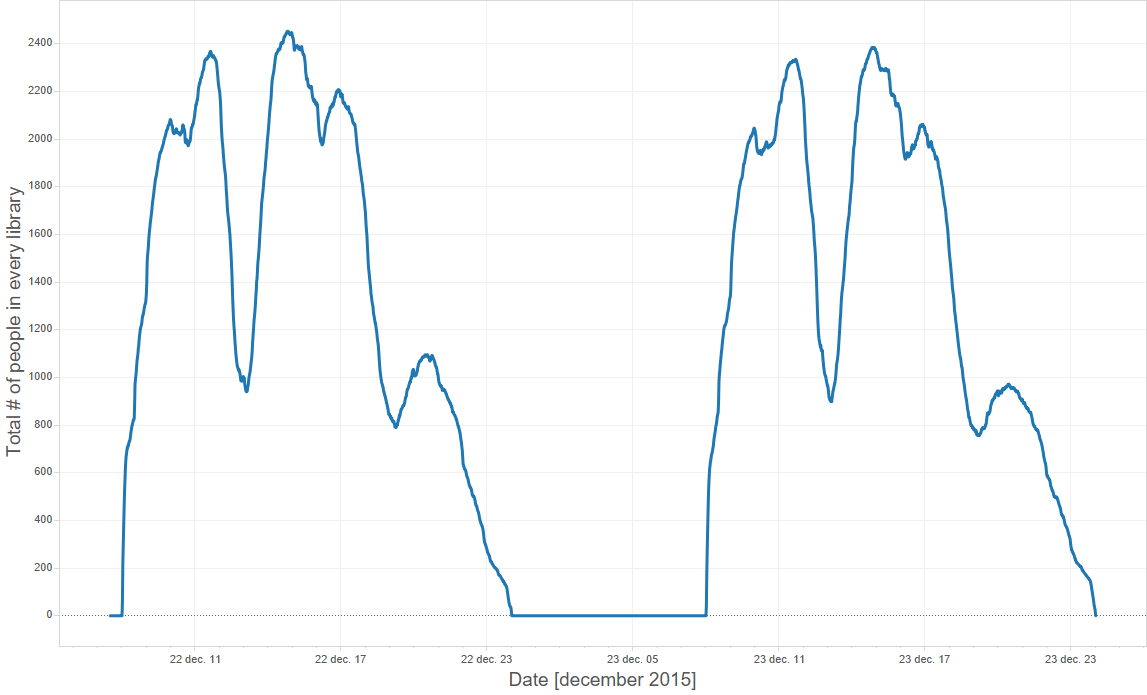
\includegraphics[scale=0.2]{total}
	\end{figure}}
\item Evaluating change detection methods:
	\only<3>{
	\begin{itemize}
	\item Probability of true change detection
	\item Probability of false alarms
	\item Delay of detection
	\end{itemize}
	}
\end{itemize}
\end{frame}

\begin{frame}
	\frametitle{Experimental Design}
	\begin{itemize}
		\item Cross-validation is not directly applicable
		\item Taking snapshots at different times
		\item Other techniques needed
	\end{itemize}

\end{frame}


\begin{frame}
	\frametitle{Evaluation of Time-Ordered Data}

	\begin{itemize}
		\item \textbf{Holdout:} keeping a subset
		\item \textbf{Interleaved Test-Then-Train:} check every instance first
		\item \textbf{Controlled Permutations:} run multiple test with permutated copies of the data
		\begin{itemize}
			\item (averaging accuracy might mask adaptation properties)
		\end{itemize}
	\end{itemize}

\end{frame}


\begin{frame}
\frametitle{Experimental Design}


\end{frame}

